\documentclass[11pt]{article}
\usepackage[utf8]{inputenc}
\usepackage[T1]{fontenc}
\usepackage{fixltx2e}
\usepackage{graphicx}
\usepackage{longtable}
\usepackage{float}
\usepackage{wrapfig}
\usepackage{rotating}
\usepackage[normalem]{ulem}
\usepackage{amsmath}
\usepackage{textcomp}
\usepackage{marvosym}
\usepackage{wasysym}
\usepackage{amssymb}
\usepackage[hidelinks]{hyperref}
\usepackage{listings}
\usepackage{xcolor}
\usepackage{amsthm}
\usepackage{subcaption}

\usepackage[backend=biber]{biblatex}
\addbibresource{references.bib}

\newcommand{\n}[0]{\\[\baselineskip]}


\author{140011146}
\title{CS4303 Practical 3}

\begin{document}

\maketitle



\section{Title}
Curry\TeX\ Studios.
\n
Curry for Haskell Curry and \TeX\ for \LaTeX.

\section{Genre}
Incremental management simulation game.


\section{Rules and mechanics}
The idea of the game is to build a start-up company to be bigger, by gaining reputation and therefore earning more money and growing the company. The core gameplay mechanic is managing how the workers work by dragging their avatar boxes to different locations to start new activities. Some activities add progress to the company, such as getting and working on new projects to gain money/reputation. Other activities include improving the workers individually, such as giving them stats. 
\n
The rest of this section explains all the various game mechanics and what they represent in terms of design and ludology.
\subsection{Player}
The player plays as a manager of a technology start-up company. The player can hire workers and manage what they do. The player can also click on either a worker portrait or a game location to speed up the workers working there. 

\subsection{World}
The world of the game exists through the eyes of the player, who has a view of everything that their workers can do and are currently doing. The interface provides the player with information, anything that is not non-deterministic is shown to the player to allow them to make decisions without hidden information. 
\n
The in-game time of the world is always ticking past, but is paused at certain times to allow the player to make an informed decision. This creates a combination of speed to assign and micromanage workers and time for the player to think about decisions. 

\subsection{Workers}
There are many mechanics to each worker:
\begin{itemize}
\item Skills
\item Stats
\item Caffine addiction
\item Stress
\item Wage
\end{itemize}
An important aspect of the game is balancing workload and the different mechanics for all workers in the company. For example, always assigning workers to work on projects increases their skills and stress and earns the company money, but assigning workers to increase their stats allows the company to earn more money and reputation in the long run. 
\subsubsection{Projects and Skills}
As the game is programming themed, each project has associated skills (languages) that are needed. Any worker can work on any project regardless of skills like in real life, but will be less efficient if they are not skilled in those languages. Working on projects increase the worker's experience and level in the project's related skills. This was chosen instead of allowing the player to manually assign skill points to workers to make it more realistic and slightly reduce the complexity of the game as there are already many systems that add complexity. The experience gained is also random to make the game less deterministic and also more realistic and people may learn more or less based on many factors when working.
\n
The player can assign workers with no skill or different skills to a project without any negative penalty and the skills matching only provides a bonus. Only the worker's best two skills are displayed and active. This was a feedback point from testing which is discussed further in section \ref{sec:testing-skills} which simplifies this mechanic because otherwise, every worker will almost always have some experience in every skill. 

\subsubsection{Stats}
Workers have two stats:
\begin{itemize}
\item Entrepreneur level
\item Fame level
\end{itemize}
These stats affect projects that the worker works on. Whenever a worker works on a project, they have a chance to increase the money and/or reputation that project generates based on these stats. Additionally, the high level these stats are, the more wage must be paid to the worker. 
\n
The design behind adding these stats is to represent a trade off. The player has to decide between assigning workers to work which generates income and reputation or spending time to improve their stats to get more money/reputation in the long run. 


\subsubsection{Coffee}\label{sec:rules-coffee}
Coffee is an additional mechanic is make the game more challenging and provide conflict to reach the goal. Workers with caffeine addiction will drink coffee when they work on projects. When they need to drink is stochastic and based on their addiction level to add predictable randomness to their behaviour. The coffee makes them a bit more productive than other workers, but they consume one coffee. If the company is out of coffee, workers who need to drink coffee regularly become more stressed and may not be able to continue to work until they get some coffee. 
\n
The player can drag workers to the cafe to get more coffee for the company. This mechanic represents a small trade off, difficulty and conflict to the game. The trade off comes when choosing new workers to hire, as the player may have to choose between a less skilled worker with less caffeine needs and a more skilled worker with more caffeine needs. The difficulty and conflict comes from needing to remember and assign workers to occasionally get coffee instead of doing productive activities and stalling and increasing a worker's stress when the company is out of coffee. 

\subsubsection{Stress}
Stress is another mechanic that adds conflict. Every time a worker does any activity, it adds to their stress levels. At 100\% stress the worker cannot do any further activities and must rest. The stress also increases the time it takes for a worker to complete an activity by exactly the stress percentage. 
\n
This gives a bit of ``downtime" for workers so they cannot always be doing productive work and for players to decide when they should let their workers rest. The amount of stress gained is random to add non-determinism.

\subsubsection{Wage}
Wage in combination with the game time are part of the ``opponents" of this game. Every worker employed by the player/company have a salary that must be paid at the end of every month. This means the player has to earn enough money every month to pay the workers. This mechanic is deterministic so that the player knows exactly what is required to not lose the game. Even more control is provided via the ability to pre-emptively pay salaries. 
\n
If the player cannot pay the wages once, the company's money goes into the negative. This is bad for the player because they cannot buy any upgrades until they get over the negative debt and will push into the next month's earnings. The player will lose the game if they still have negative money at the start of the next month. 


\subsection{Money and reputation}
Both money and reputation play a key role in the game. Reputation is the end goal and win condition of the game and money helps to both reach that goal and prevent the player from losing. To win the game, the player must help the studio reach a certain number of reputation by 1 year. The player will lose the game if they do not reach this goal or are unable to pay worker wages (start the month with negative money) at the start of every month. 
\n
There are again more trade offs here. Money is used to pay wages and also buy upgrades and hire new workers, which allows the player to progress and expand the company while reputation is the final goal so it cannot be ignored. Additionally, more reputation increases the money that project gives. This is to reward players who wish to focus on gaining reputation, ensuring progress so players aren't punished for trying to reach the goal rather than earn money and as a bit of realism since a more known company should be able to find higher paying projects. 
\n
The kind of projects that are generated reflect the trade off as well. For example, some projects earn the player a lot of money, but give negative reputation and there are projects which earn no money, but give much more reputation. 


\subsection{Upgrades}
Upgrades serves as an important aspect of the game for progression, allowing the player to hire more workers and get to the goal more easily. Upgrades are a way for players to spend money to progress faster and reach the goal. 
\n
There is a maximum amount the upgrades can be purchased as the game is not expected to last for much longer. The way the upgrades increase cost and benefit is based on an article \cite{upgrades} on incremental games and their formulas.


\section{Context}
The game is based on a small mixture of genres: incremental clicker games like Cookie Clicker \cite{cookie} and business simulation games where micromanagement of the workers is emphasised.

\subsection{Similarities and differences}
The clicking aspect of the game to speed up progress and being able to progressively unlock more workers and earn more money is a concept taken from incremental games. However, unlike incremental games, this game is not automatic and requires lots of decision making and micromanagement, which is where the similarities with business simulation games come in. 
\n
On one hand, there are many features such as worker skills which affect time taken to work and are gained by working on projects rather than being assigned by players which attempt to accurately simulate the real world as part of simulation genre. However on the other hand, mechanics like clicking to speed up workers and managing everything workers do including rest is unrealistic but make the game more fun and accessible, for example otherwise the player would only be managing workers for a third of each day. 
\n
Other games with the same genre and theme include Game Dev Tycoon \cite{game-dev-tycoon} and Whipbit Solutions \cite{whipbit}. Although this game has many similar concepts with those games, many design decisions such as how the skills/stats are gained and how clicker aspects were introduced make this game different from an exact clone of those games.

\section{Design}
This section aims to cover specific aspects of the game design of note or aspects that have changed over the course of developing and testing the game with other people.

\subsection{Game time}
Time is very important in this game because it is the main opponent and driving factor behind player decisions on what their workers should be doing. For this reason, the game is only updated based on the \texttt{GameTime} and the \texttt{GameTime} is updated independent of the frame rate and based on real time. The implementation details can be found in the code and documentation and is based on an article \cite{time} by Glenn Fiedler. 
\n
This approach solves two issues:
\begin{enumerate}
\item Fluctuating game time due to frame rate issues.
\item Cheating by changing the speed at which the game is run at to get an advantage. 
\end{enumerate}
Solving both issues ensures the game is played on a level playing field, where success is based on a player's strategy and a bit of luck from the non-deterministic aspects of the game. 

\subsection{Cheating}
Except for game time being independent, there are many ways to cheat in this game. The most obvious is to set up some kind of script or auto-clicking program to play the game. Now it is difficult to prevent auto-clicking software from cheating, but I have included many non-deterministic aspects in order to prevent script cheating as much as possible. 
\n
Because many aspects of the game such as stress gain, random project and worker generation are stochastic, it makes it more difficult to write a simple script to play the game. It does not stop this cheating entirely, but a more complex script may be needed to play this game effectively.

\subsection{Locations and player clicking}
The idea behind allowing players to put multiple workers in a single location and click the location to decrease the work timers of all workers there is to provide micromanagement decisions on tasks for workers to do. It is more optimal for the player to put all workers on the same tasks so they can decrease their timers all at once, but often the player may find many different activities have to be worked on concurrently. 

\subsection{Testing and evaluation}
I have tested my game with a few other students and there were multiple design points that were altered or adjusted based on their feedback. Some adjustments were small quality of life or interface changes that will not be detailed in this report. The changes that are documented are those that affected certain design or mechanics of the game. The main points that were tested for opinion from others is the difficulty of the game and whether the systems and mechanics were intuitive to understand. 
\n
As a general note, the game was often found to be quite difficult and the systems and mechanics not easy to understand unless I explained them. As a result, I have added information boxes and improved the UI as much as possible to explain the game concepts in game as well as change the numbers to make the game easier.

\subsubsection{Incremental progress}
A point brought up by a few people was that there is initially too many mechanics in place at the start of the game and players often felt overwhelmed on what they should be doing. This also meant that the more important activity (getting and working on projects) was less emphasised because the player was trying to learn all the mechanics at once rather than knowing which aspect is more important to focus on.
\begin{figure}[H]
\centering
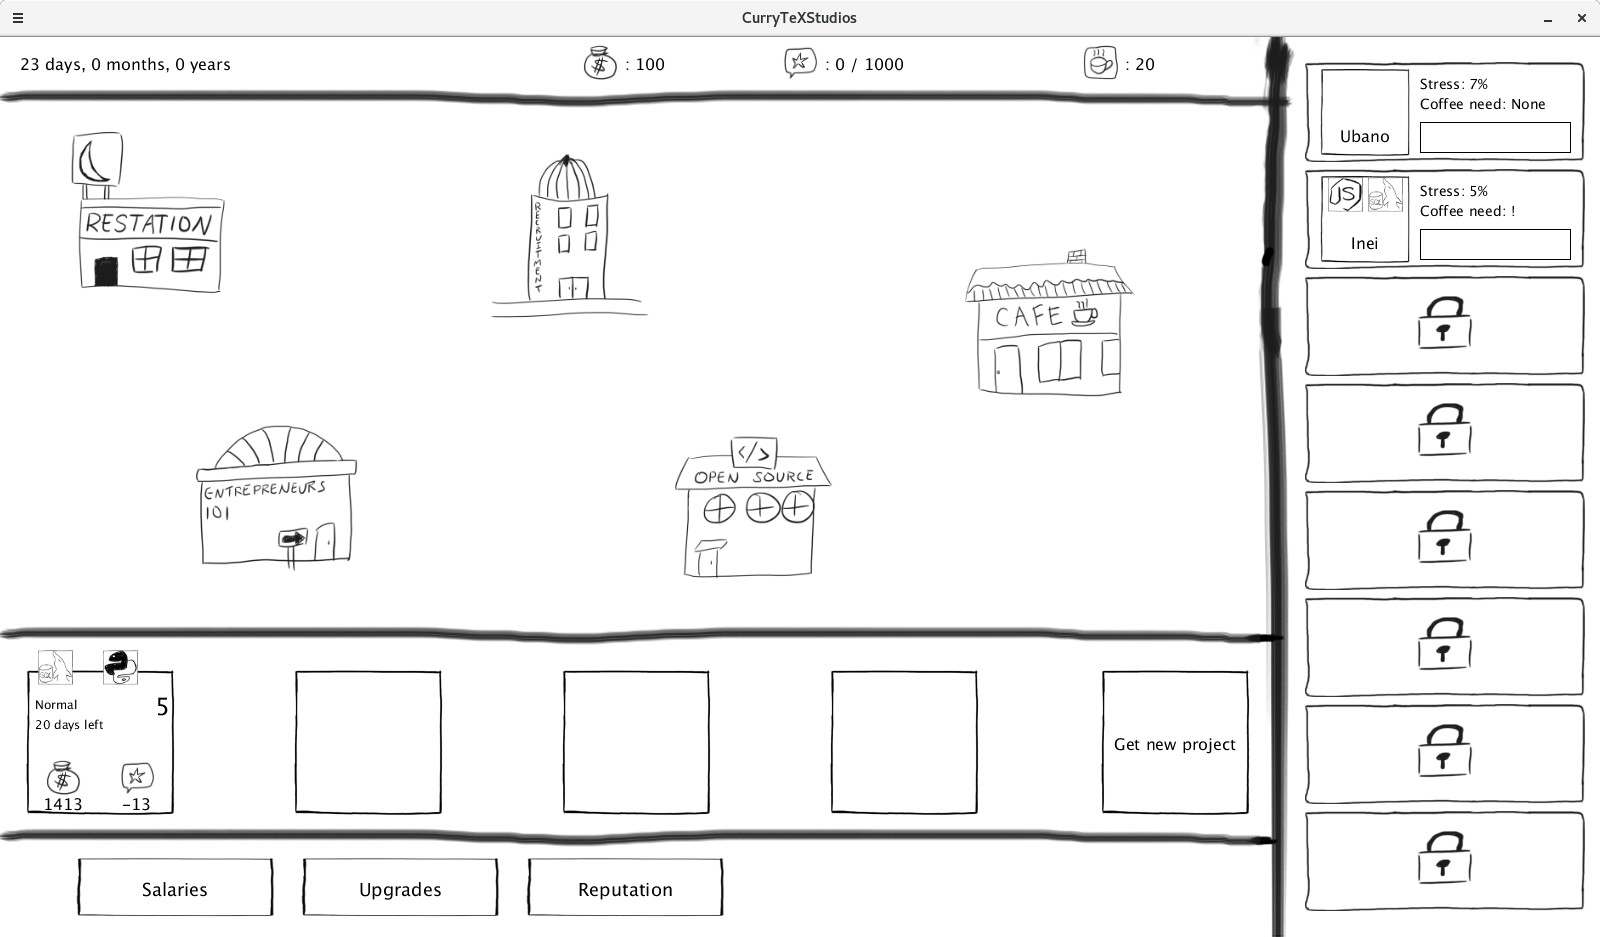
\includegraphics[width=1\textwidth, keepaspectratio]{imgs/all-features.png}
\caption{Game with all features available}
\end{figure}

\begin{figure}[H]
\centering
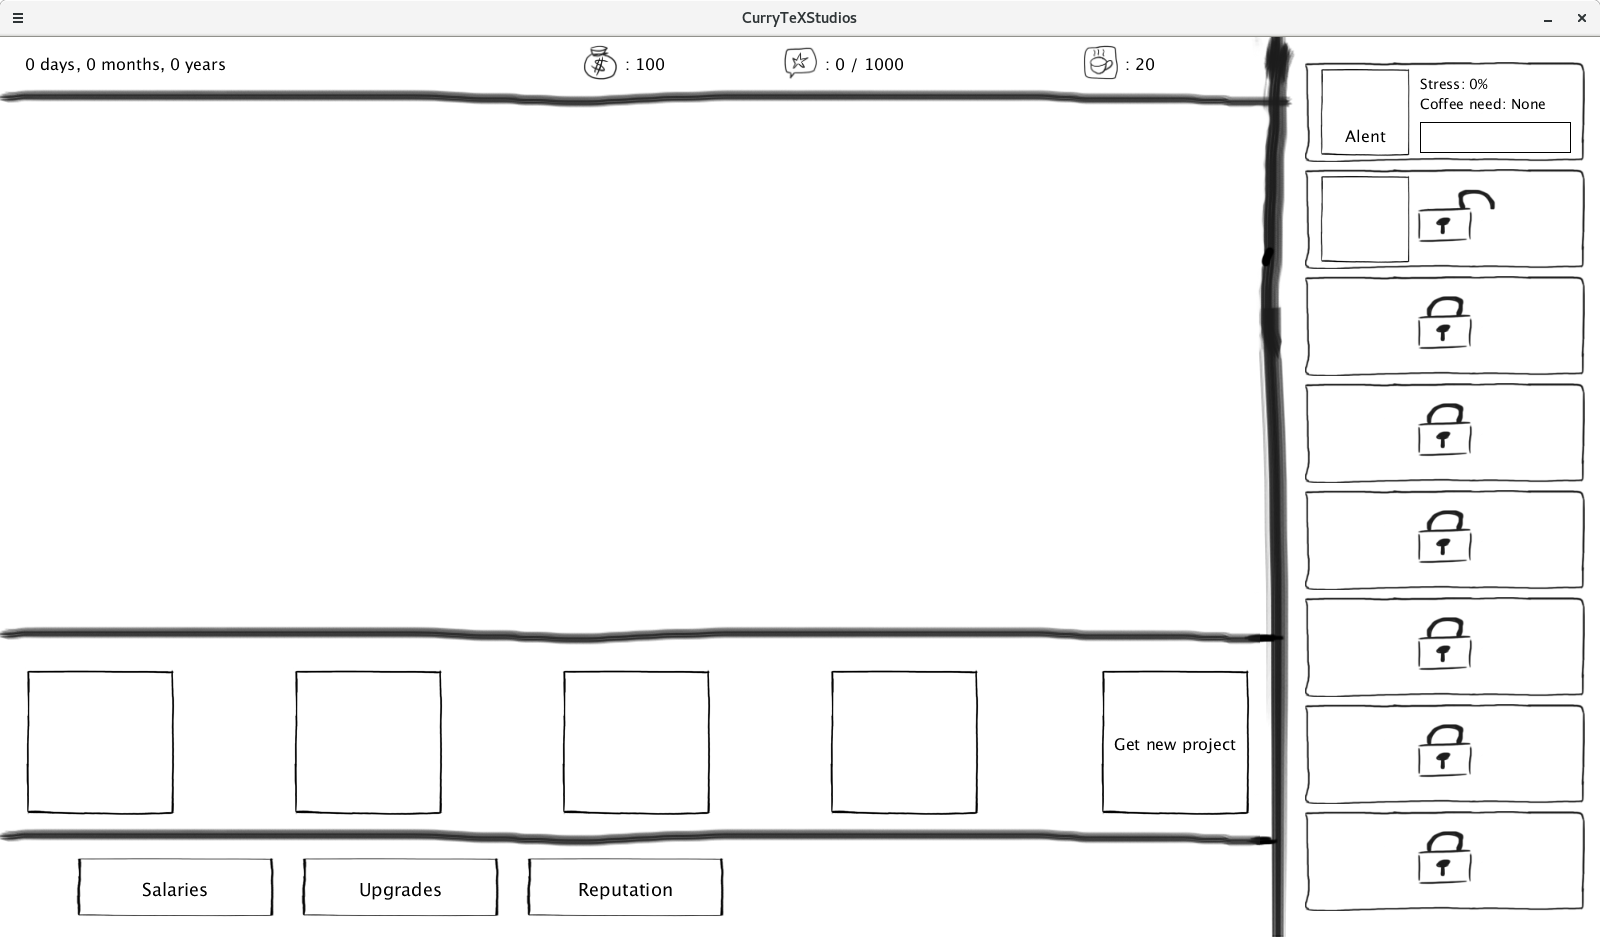
\includegraphics[width=1\textwidth, keepaspectratio]{imgs/no-features.png}
\caption{Game with only the very basic mechanic shown}
\end{figure}
\noindent
The change based on this feedback was to incrementally introduce all the features and mechanics of the game so that the player was given more time to adjust and learn how to play the game. The change meant that at the start of the game, the player can only assign workers to get and work on projects without worrying about any other mechanics. As the game time progressed, the other mechanics are shown and introduced so the player can try them, for example the coffee mechanic is only told to the player after they hire a worker who needs coffee and the ability to hire a new worker is not introduced until a few in-game days. 

\subsubsection{Skills mechanic}\label{sec:testing-skills}
Initially, all of a workers skills and levels were displayed and they all affected the worker's speed when working on a project. This made matching a worker to an appropriate project more difficult because every skill was listed and it was not immediately clear which was the skill the worker was best at. Furthermore, because of the nature of gaining experience on skills when working on projects, games usually ended up with all workers having all skills at different levels. This issue was brought up when testing with other students as they found when playing they did not pay much attention to the skills mechanic because of both its complexity and its lack of reward/punishment. 
\n
To improve on this, the speed gained when working on a project with matching skills was increased and only the two best skills for a worker is taken into account when applying this matching. The best skills are determined to be the two skills a worker is most proficient at (highest level and experience). This also does not take much away from the realism, as programmers may know many different languages, but are often skilled only in a small handful. If a worker becomes more skilled in a language, that language will overtake and become one of the worker's top two. 
\begin{figure}[H]
\centering
\begin{subfigure}{.5\textwidth}
\centering
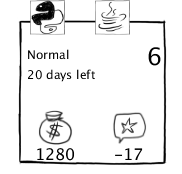
\includegraphics[width=0.6\textwidth, keepaspectratio]{imgs/project.png}
\caption{A project box}
\end{subfigure}%
\begin{subfigure}{.5\textwidth}
\centering
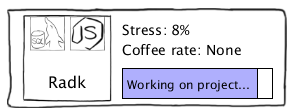
\includegraphics[width=0.7\textwidth, keepaspectratio]{imgs/worker.png}
\caption{A worker box}
\end{subfigure}
\caption{The project and worker interface elements, showing the language icons to allow players to more easily identify and match them accordingly.}
\end{figure}
\noindent
Additionally, the interface was changed along with this design change. Because now each worker only has two associated skills that need to be displayed, the language icons can be displayed on the worker boxes. The visual icon makes it easier for players to match workers to projects. 


\subsubsection{Coffee mechanic}
Another mechanic that was changed was the way the coffee affected a worker's productivity. Before any changes, the coffee had no positive affect and the negative affects were causing the worker to gain more stress if they could not drink coffee and slightly increase the time of their current activity. The people who played the game noted that the coffee mechanic did not have enough of an effect on the game, meaning it was mostly ignored. 
\n
To address this and make the coffee cause more of a challenge and conflict, a small benefit and greater punishment was added. The details of the mechanic was detailed earlier in section \ref{sec:rules-coffee}. 

\subsubsection{Stress mechanic}
Before the changes, stress was a simpler and deterministic aspect of the game. Each activity always gave the percentage increase to stress and the only negative part about stress was the inability to work at 100\%. Players who have tried my game said that this meant they rarely cared about the stress levels, only resting their workers when they needed and in general not paying a lot of attention to it.
\n
To increase the impact of stress, the amount of stress gained changed to become non-deterministic and the stress directly and negatively affected the time it took a worker to complete a task. The effect of this could be clearly seen in the game as a worker who was more stressed clearly worked slowly than a worker with less stress. The non-deterministic aspect provides more conflict so the player cannot easily predict and plan ahead when and how to rest workers most efficiently. 

\subsection{Further work}
Given more time, the most important aspects I would like to work on are improving the interface so more information is easily available and so what actions the player can do is more intuitive and balancing the numbers in the game so it is fairly challenging but not overly difficult, especially to new players.
\n
More features that increase the complexity of the game, such as items which increase a worker's speed or speed only on certain languages could be added, but such features would have less priority over balancing the game and improving the interface. 

\section{Platform}
The game was developed for a desktop computer, but the mechanics are done such that it could be ported and be suitable for a tablet device.

\section{Acknowledgements}
The code for dragging boxes around is adapted from \cite{drag} and the code for animating images is adapted from \cite{animation}.

\printbibliography

\end{document}

